

\section{Setup of the Base System}

The base system consists of a standard raspbian operating system, the EIBD daemon, shared libraries which are used by EIBD and the master daemon.
The operating system is based on the Debian project, with the kernel, libraries and binaries ported to the ARM platform, so it is possible to benefit from
using a full-scale operating system, e.g. by using the comfortable packet manager called
\textit{aptitude} provided by Debian. A short introduction to the most important commands is given below as they are needed.

\subsection{Raspbian}

To obtain a running system for deploying the secure KNX daemon, a prebuilt Debian image is used, which can be ownloaded from the raspberry homepage:

\url{http://downloads.raspberrypi.org/raspbian_latest.torrent}

The image must be unzipped and copied to a suitable memorycard. First-generation raspberries(model 'A') have SD slots, while
all later models come with micro-SD slots. To copy the basic operating system to the memorycard, the linux commandline tool 'dd' can
be used. To find the correct device to write the image to, the following command can be used: 

\begin{lstlisting}[style=BashInputStyle,label=lst:kern.log]
    # tail -f /var/log/kern.log
\end{lstlisting}

After inserting the memorycard into a cardreader, look for output like that:

\begin{lstlisting}[style=BashInputStyle]
    [1004111.533698] sdb: detected capacity change from 7909408768 to 0
    [1004114.055840] sd 6:0:0:0: [sdb] 15448064 512-byte logical blocks: ...
\end{lstlisting}

Here, the proper device to use is the device /dev/sdb.
\textbf{Pay attention to use the correct device in the following command - this device will be overwritten}:

\begin{lstlisting}[style=BashInputStyle]
    # dd if=<Path to Image> of=<Device to overwrite>
\end{lstlisting}

After the write command has finished, the memory card is ready to use. For first time setup, a display must be connected via HDMI. Powering up the raspberry
opens a ncurses configuration dialogue. First thing to do is to resize the root partition to maximum size and set a password for the administrative
account. Optionally, different options like keyboard layout can be set.
To be able to operate the raspberry without external display, it is necessary to start the \gls{ssh} server under \textit{Advanced Options} and assign a 
fixed ip to the host by editing the file \textit{/etc/network/interfaces}, as shown in example \ref{lst:staticIP}. This way it is possible to connect to the
raspberry with a \gls{ssh} client. For password less logins, create an unpriviliged user and
 a \gls{ssh} public/private key pair for that user by executing these commands on the raspberry pi:

\begin{lstlisting}[style=BashInputStyle]
    # groupadd <usergroup>
    # useradd -g <usergroup> -m <username>
    # su <username>
    # ssh-keygen
\end{lstlisting}
 
The program generates the user and the correspoding key pair and saves public and private key in the subdirectory ~/.ssh/ on the actual host. When asked for a passphrase, it is possible
to use a password-less keypair, an option that should only be used in restriced areas.
To actually use the keypair for logging into
the raspberry pi, the public key must be saved in the file \textit{~/.ssh/authorized\_keys}. Additionally, the private key must be copied to every host
from that \gls{ssh} connections to the raspberry pi want to be opened. After that, it is possible to load the private key into memory with the command \textit{ssh-add}
and to connect to the host without a password:

\begin{lstlisting}[style=BashInputStyle]
    # ssh-add // only necessary when non-empty passwort is used for keypair
    # ssh <username>@<host-ip|host-dns-name>
\end{lstlisting}

It is also advisable to update the operating system at this time by running the following commands as user root:

\begin{lstlisting}[style=BashInputStyle]
    # apt-get update
    # apt-get install
\end{lstlisting}

This will install the latest package versions of all installed packages. New software can be installed from the command line with these commands:

\begin{lstlisting}[style=BashInputStyle]
    # apt-cache search <pattern> // print a list matching packages for <pattern> 
    # apt-get install <packagename>
\end{lstlisting}

\subsection{EIBD}

The maintainer of EIBD only provides binary packages for the i386 architecture, so the daemon and its prerequisites must be built from source to get
suitable binaries and shared libraries for the ARM environment. Building software under GNU Linux or *nix from source always follows this scheme:

\begin{enumerate}
 \item Downloading and extracting the source code
 \item If possible, comparing the developer supplied hash code  with the hash code of the downloaded source files with
 \textit{sha256} or one of its variants to verify that no modified software has been downloaded.
 \item Optionally, apply patches to the source code(not necessary here).
 \item Set the make-options by calling \textit{./configure <options>}, overriding default compilation options by setting the corresponding command line parameters.
 \textit{./configure --help} should print a list of valid options.
 \item Compiling the source code by calling \textit{make}.
 \item Copying the generated binaries and shared libraries into their correct place by calling \textit{make install}. This last step must always be executed
 as user root because the generated files will be copied into system directories which are not writeable by unprivileged users.
\end{enumerate}

EIBD and the needed library \textit{pthsem} are available from these locations:

\url{https://www.auto.tuwien.ac.at/~mkoegler/pth/pthsem_2.0.8.tar.gz}
\url{http://sourceforge.net/projects/bcusdk/}

After copying the archives to the raspberry, they must be unpacked and compiled. First the pthsem shared library, which offers user mode multi
threading with semaphores, must be compiled because it is used by EIBD. 

\begin{lstlisting}[style=BashInputStyle]
    # tar -xvzf pthsem-2.0.8.tar.gz
    # cd pthsem-2.0.8
    # ./configure
    # make
    # make install // must be executed as root
\end{lstlisting}

This will, among other things, generate the shared library \textit{libpthsem.so.20} in the directory \textit{/usr/local/lib}. \textit{/usr/local}
 is by convention the destination where self compiled software should reside.
Now that pthsem is available, which is a dependence of the EIBD daemon, EIBD itself is ready for compilation:

\begin{lstlisting}[style=BashInputStyle]
    # tar -xvzf bcusdk-0.0.5.tar.gz
    # cd bcdusk-0.0.5
    # ./configure --without-pth-test --enable-onlyeibd --enable-tpuarts
    # make
    # make install // must be executed as root
\end{lstlisting}

These steps generate the binary \textit{eibd} and lots of helper programs in the directories \textit{/usr/local/bin}, and the shared object
\textit{/usr/local/lib/libeibclient.so.0} that provides the \gls{eibd} \gls{api} and therefore is needed to be linked to the master daemon. 

\subsection{Revision control}

The source of the master daemon is managed by GIT. GIT is a decentralized revision-control system and is available under Debian/Raspbian after installing
the package 'git'. The command \ref{lst:git} fetches the latest version and creates a directory called 'knxSec' which contains all the needed source files,
a proper makefile \ref{lst:makefile} for the project, as well as all other needed files.

\begin{lstlisting}[style=BashInputStyle,label=lst:git]
    # git clone git@github.com:hglanzer/knxSec.git
\end{lstlisting}

\subsection{Busware \gls{usb} couplers}

To make the KNX TP1 bus accessible, i.e. to write datagrams to and receive datagrams from the bus, \gls{usb} dongles as shown in figure \ref{fig:busware}
from the company \textit{Busware} are used. Depending on the revision, the bus couplers creates a new device which is used as \gls{url} by the \gls{eibd}.
The coupler will be accessible by \textit{/dev/ACMx}, where x is the number of the device. It may be necessary to flash the bus couplers with the correct
firmware first. The easiest way to check this is to use command \ref{lst:kern.log} and look for output similar to listing \ref{lst:device} when plugging 
the coupler into an \gls{usb} slot.

\begin{lstlisting}[style=BashInputStyle,label=lst:device]
... usb 1-1.2: new full-speed USB device number 19 using ehci_hcd
... usb 1-1.2: New USB device found, idVendor=03eb, idProduct=204b
... usb 1-1.2: New USB device strings: Mfr=1, Product=2, SerialNumber=220
... usb 1-1.2: Product: TPUART
... usb 1-1.2: Manufacturer: busware.de
... usb 1-1.2: SerialNumber: 7543034373135130C140
... cdc_acm 1-1.2:1.0: ttyACM0: USB ACM device
\end{lstlisting}

If no such line like 7 appears, the correct firmware is available as file \textit{firmware/TPUARTtransparent.hex} inside the git project. To actually flash the 
coupler, the programming button on the bottom of the device must be kept pressed while connecting it to an \gls{usb} slot. Afterwards, the commands shown
in \ref{lst:flash} must be executed.

\begin{lstlisting}[style=BashInputStyle,label=lst:flash]
    # apt-get install dfu-programmer
    # dfu-programmer atmega32u4 erase
    # dfu-programmer atmega32u4 flash TPUARTtransparent.hex
    # dfu-programmer atmega32u4 reset
\end{lstlisting}


\begin{figure}
    \centering
    \caption{Busware KNX-USB coupler}
    \label{fig:busware}
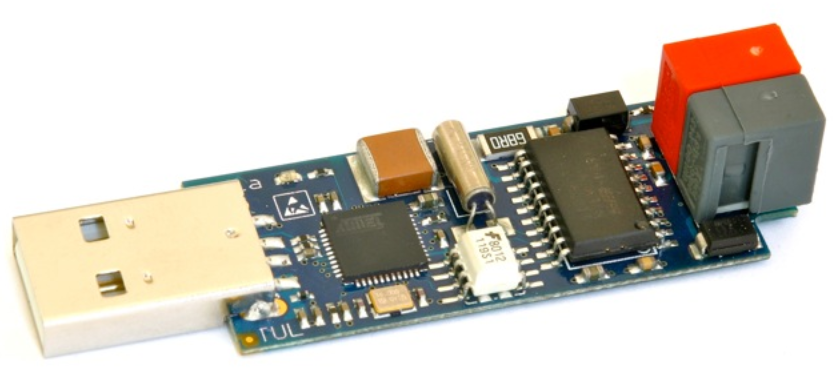
\includegraphics[scale=0.2]{figures/busware.png}
\end{figure}

\subsection{Test setup}

The test environment consists of 2 raspberry pis, as shown in figure \ref{fig:secArea}. 

\section{Master daemon}



